
\section{Hierarchical Data Model Mapping}
\label{sec:histo.hierarchy}
Our data described in the scenario is structured through entity instances, their attribute values and relationships to other instances.
Most modern web application frameworks realize one-to-one relationships by simply having an attribute storing the related instance's ID.
One-to-many relationships are realized through an attribute having a collection of 
instance IDs as its value.\\
Instance collections often have a relevant order that needs to be preserved.
An example is the list of tasks in a project that is displayed to the user.
The user wants to be able to change the order of tasks and the order should be persisted.\\
We further differentiate between linking to a separately stored instance and  embedding an instance.
An embedded instance can still be linked from other instances but it cannot be embedded twice.
Linking to an instance means to simply hold another instance's ID as an attribute value, embedding means to hold both their ID and actual state.\\

The merge and commit processes, described in the next sections, depend on a hierarchical representation of our application state.
To have a hierarchy we need to define a single root structure from where all substructures of our state can be reached.\\
Our hierarchical structure can be as simple as this:

\begin{itemize}
\item Level 0 (Root): list of entities
\item Level 1: list of instances per entity
\item Level 2: list of attributes per instance
\end{itemize}

This gives us a very flat tree with each entity node linking to a potentially large number of instances.
For example, our comments entity would directly link to all comments across all projects and tasks.
The next sections will show that it is beneficial for merging performance if each tree node only links to a small number of child nodes.\\
This is where the difference between linking and embedding comes into play.
We can achieve a deeper hierarchy by embedding certain instances in others.
In our scenario we could decide to embed tasks inside projects through one of its attributes.
Comments could in turn be embedded inside tasks.\\
In order to develop a merging algorithm we need to map each substructure of our hierarchy to a suitable data structure.\\
Starting at the top we choose the list of projects as the root structure of our data.
The project list is represented through a \emph{dictionary} embedding all project instances.
The dictionary keys are the instance IDs and the dictionary values embed the actual instances.\\
Each instance is again represented through a \emph{dictionary}.
The dictionary keys correspond to the attributes and the dictionary values to attribute values.\\
If the attribute values are atoms, the hierarchy stops here.
Attributes with string values can be represented with \emph{ordered lists}.
Attribute values linking to other instances are represented through \emph{(ordered) sets}.
We can choose a set as the list can only contain unique instance IDs.\\
Attribute values embedding other instances are represented through an \emph{(ordered) dictionary}.
Like in our project list at the beginning, keys are the IDs of instances and values their actual state.\\
If other instances are embedded, they are kept as children in the hierarchy.\\

Let us summarize the full mapping between model elements and data structures:

\begin{itemize}
\item Instances and their attributes: dictionaries
\item String values: ordered lists
\item Collections linking to instances: (ordered) sets
\item Collections embedding instances: (ordered) dictionaries
\end{itemize}

\begin{figure}[hierarchy]
  \centering
  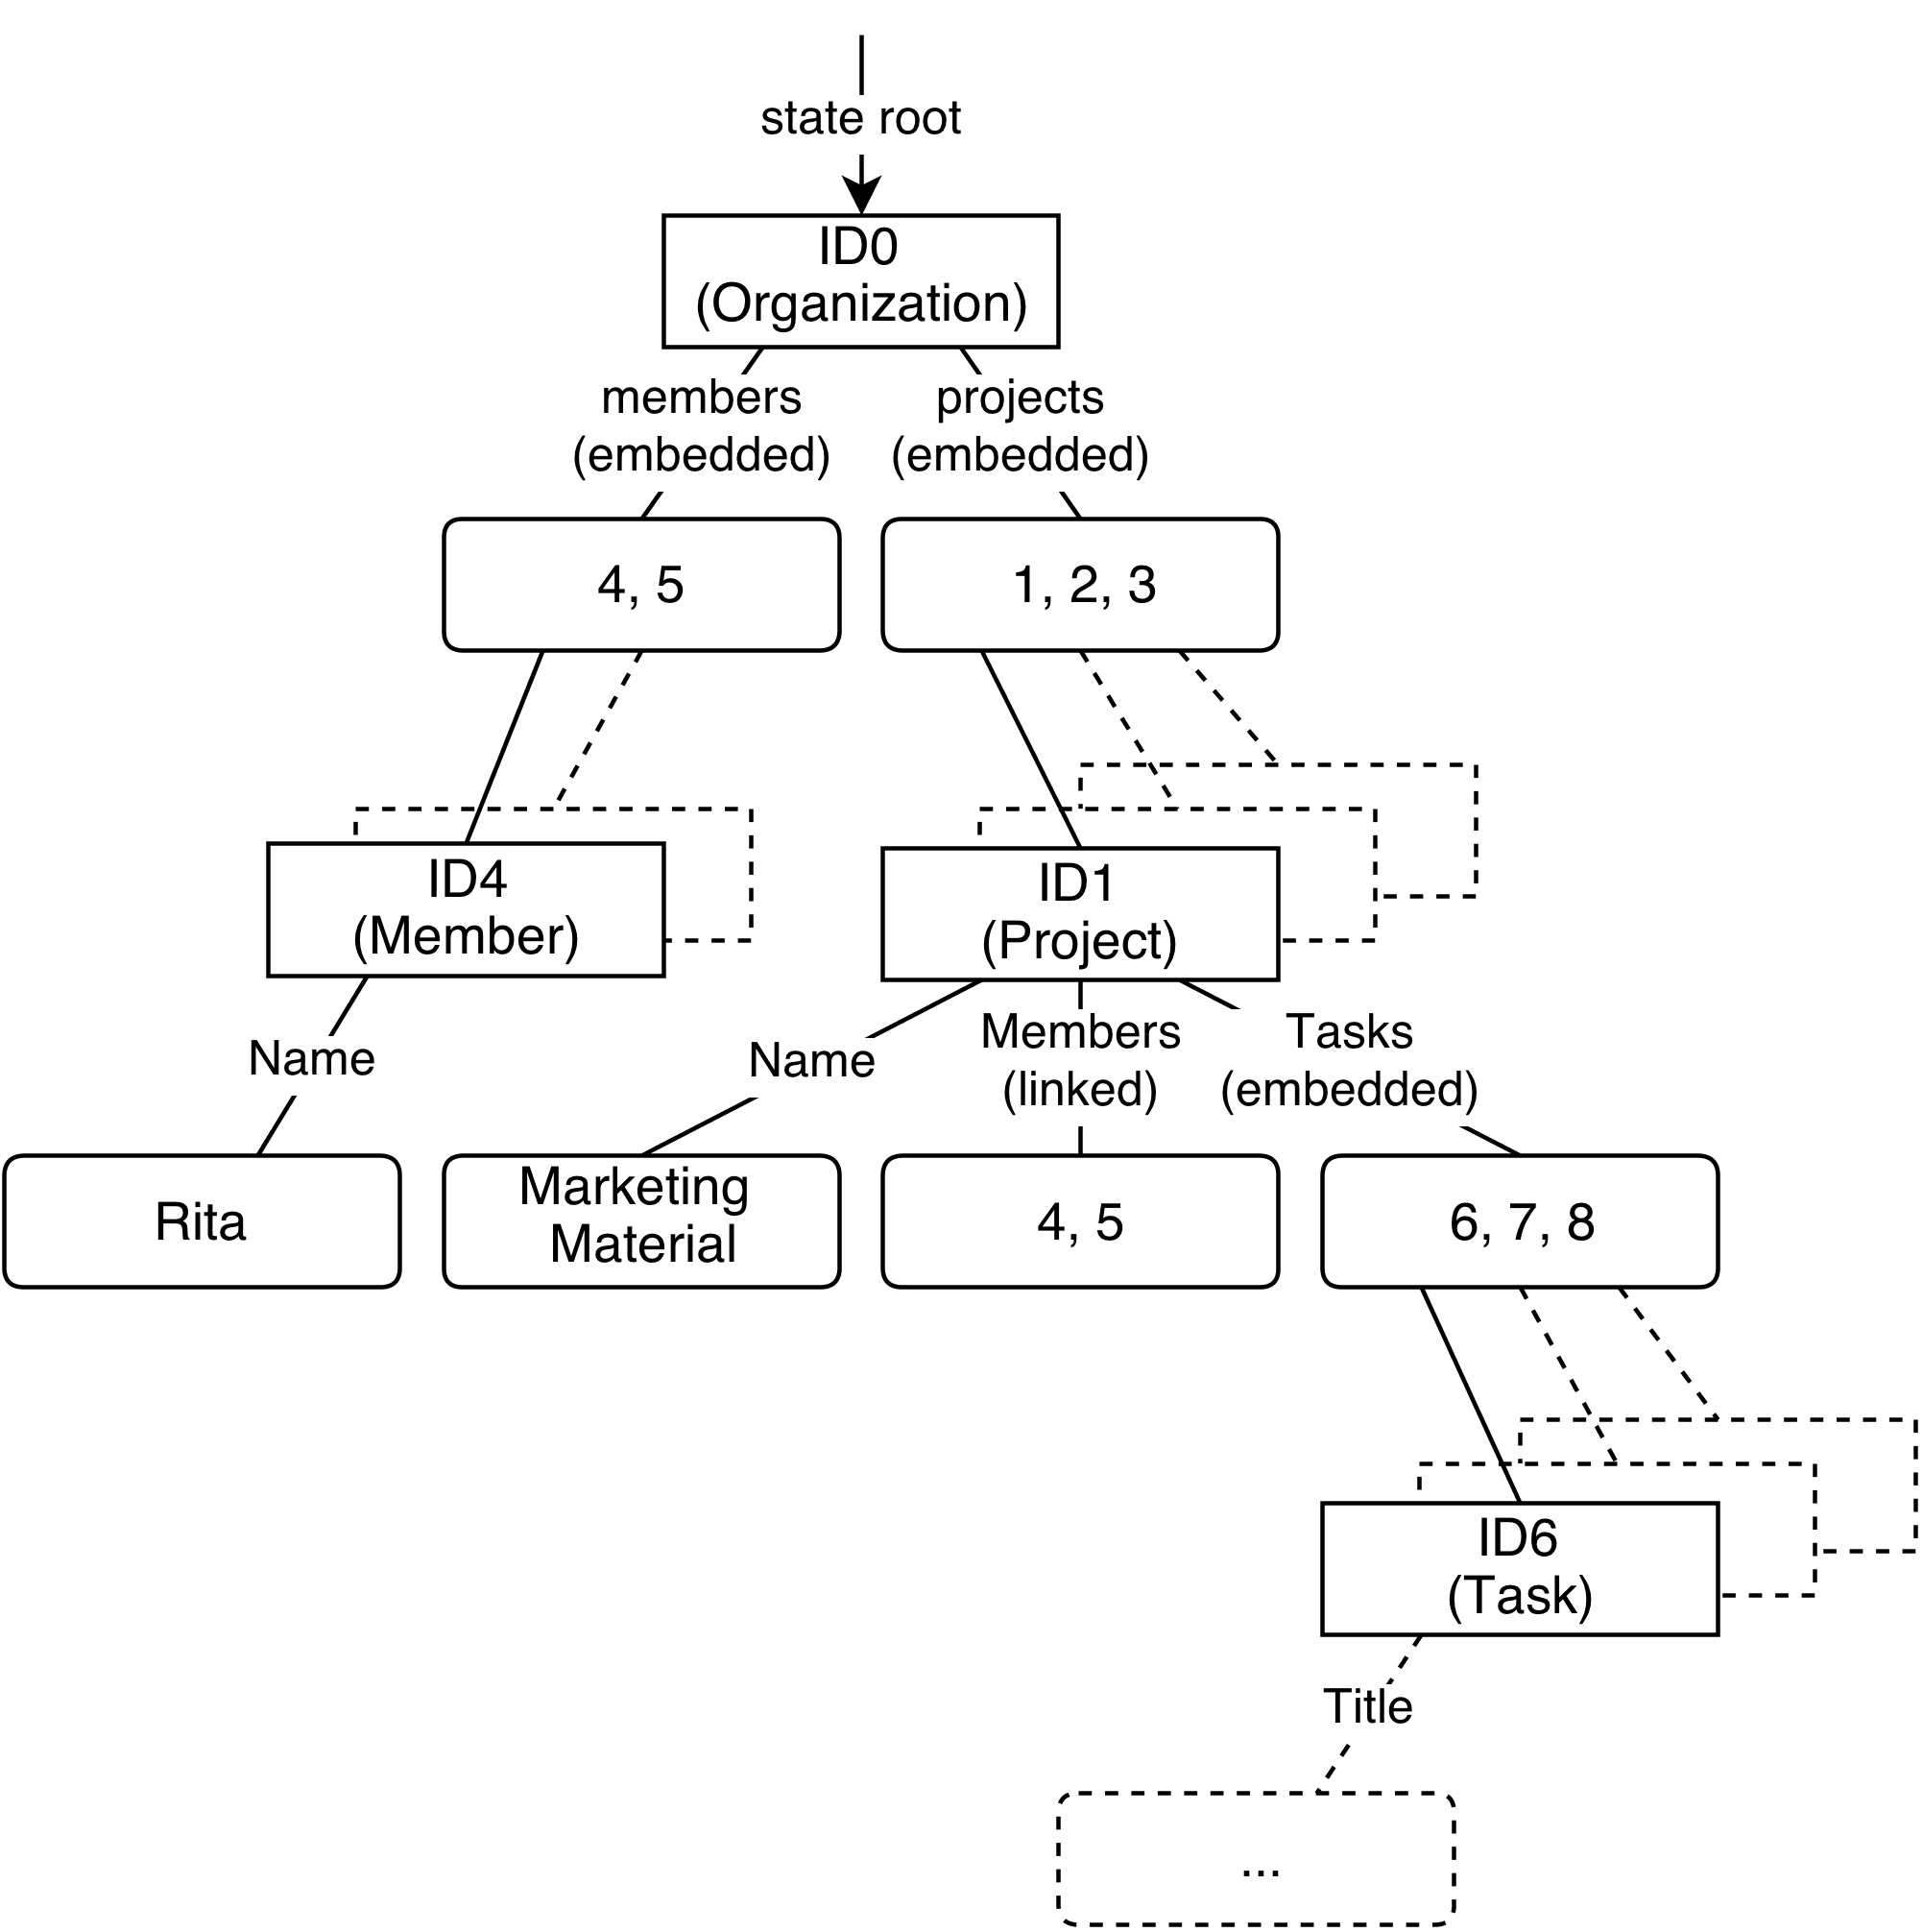
\includegraphics[width=0.8\textwidth]{img/hierarchy}
  \caption{The data model mapped to a hierarchy.}
  \label{fig:histo.hierarchy}
\end{figure}

Figure \ref{fig:histo.hierarchy} shows the actual hierarchy we derived from the data model in our scenario.